%%%%%%%%%%%%%%%%%%%%%%%%%%%%%%%%%%%%%%%%%%%%%%%%%%%%%%%%%%%%%%%%%%%%%%%%%%%%%
%	e-Yantra, IIT-Bombay

%	Document Author: Saurav Shandilya
%	Date: 16-August,2012
%	Last Editted by: Saurav
%   Date Last updated: 31-05-2016 

%%%%%%%%%%%%%%%%%%%%%%%%%%%%%%%%%%%%%%%%%%%%%%%%%%%%%%%%%%%%%%%%%%%%%%%%%%%%%

\documentclass[11pt,a4paper]{article}

\usepackage{graphicx}
\usepackage{float}
\usepackage{hyperref}
\title{Interface Ultrasonic Sensor with R-Pi}
\author{Akshit Gandhi \\ Keyur Rakholiya}
\date{\today}

\begin{document}
	\maketitle
	\newpage
	\tableofcontents
	\newpage
	\section{Tutorial Name}
		Interfacing Ultrasonic sensor with Raspberry Pi.
		\paragraph{•}
		\textbf{Objective}
		\paragraph{}In this tutorial we will be going through on how to interface an ultrasonic sensor with R-Pi. The Ultrasonic Sensor which we will be using is the HC-SR04. The HC-SR04 sensor cannot be directly used with the R-Pi, we need a voltage divider circuit, the reason will be explained in the later sections.
		\paragraph{•}The reason for using ultrasonic sensor with the quadcopter setup is that, when flying indoors autonomously we need some sort of sensor that will provide the altitude details of the quadcopter, we know that the APM 2.6 has the \textbf{Barometer Sensor}, but the limitation is that it is accurate only above 5 meters height (altitude). So, we need an Ultrasonic Sensor for height (altitude) measurement.
		\paragraph{•}We also tried interfacing the \textbf{Sonar Sensor} which is compatible with the APM 2.6. The Sonar we used is the [Maxbotic Sonar MB-1200 series]. But it didn't give us the desired results. So, we moved onto using the HC-SR04.
	\section{Prerequisites}
		Knowledge of voltage divider circuit.
	\section{Hardware Requirement}
		R-Pi, wires, HC-SR04 sensor, 1000 Ohm and 680 Ohm resistances (1 each)
	\section{Theory and Description}
		\subsection{Connecting to R-Pi}
			Powering the module is easy. Just connect the +5V and Ground pins to Pin 2 and GPIO21 on the Pi’s GPIO header.
			\begin{figure}[h]
				\centering
				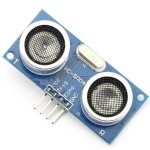
\includegraphics[scale=0.75]{sensor}
				\caption{HC-SR04 Sensor}
			\end{figure}

\paragraph{}The input pin on the module is called the “trigger” as it is used to trigger the sending of the ultrasonic pulse. Ideally it wants a 5V signal but it works just fine with a 3.3V signal from the GPIO. So we connected the trigger directly to GPIO20 on our GPIO header.
\paragraph{}
You can use any GPIO pins you like on your RPi but you will need to note the references and amend your Python script accordingly.
\paragraph{•}
The module’s output is called the “echo” and needs a bit more thought. The output pin is low (0V) until the module has taken its distance measurement. It then sets this pin high (+5V) for the same amount of time that it took the pulse to return. So our script needs to measure the time this pin stays high. The module uses a +5V level for a “high” but this is too high for the inputs on the GPIO header which only like 3.3V. In order to ensure the Pi only gets hit with 3.3V we can use a basic voltage divider. This is formed with two resistors.
\paragraph{•}
If R1 and R2 are the same then the voltage is split in half. This would give us 2.5V. If R2 is twice the value of R1 then we get 3.33V which is fine. So ideally you want R2 to be between R1 and R1 x 2. But we used 1000 and 680 ohm resistors (Because it worked the best for us!).
\paragraph{•}
Here is a diagram of our final circuit. We chose GPIO20 and GPIO16 [echo], but you can use any of the available GPIO pins on the GPIO header. Just remember to update the script.
	\begin{figure}[h]
	 	\centering
		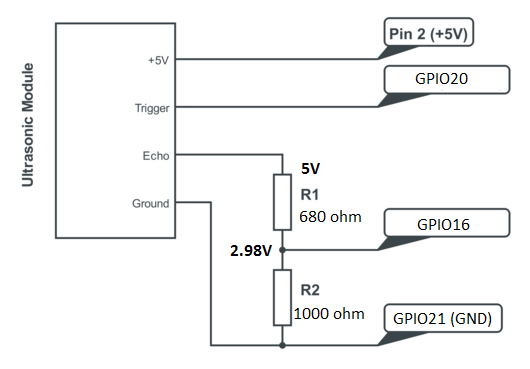
\includegraphics[width=7cm,height=5cm]{pin}
		\caption{Circuit Diagram}
	\end{figure}
	\subsection{Python Script}
		Once you have followed above connection diagram you can test the sensor you are ready with the next part i.e to access the sensor values using the python script. The script is in the codes folder.
	\subsection{Accuracy}
		\begin{itemize}
			\item The accuracy of the distance measurement is dependent on timing. Python under Linux is not ideal for precise timing but for general messing about it will work OK. To improve accuracy you would need to start looking at using C instead.
			\item When the GPIOs are configured the module needs some time before it is ready to take its first reading so we added a 0.5 second delay to the start of the script.
			\item The transducers have a wide angle of sensitivity. In a cluttered environment you may get shorter readings due to objects to the side of the module.
			\item Measurements work down to about 2cm. Below this limit the results can give strange results.
			\item If the ultrasonic transducers touch anything the results are unpredictable.
		\end{itemize}
	\section{References}
		For more understanding you can visit the below two sites:
		\paragraph{•}
			\url{http://www.raspberrypi-spy.co.uk/2012/12/ultrasonic-distance-measurement-using-python-part-1/}
			\paragraph{•}
			\url{http://www.modmypi.com/blog/hc-sr04-ultrasonic-range-sensor-on-the-raspberry-pi}
	
\end{document}



